
% This LaTeX was auto-generated from MATLAB code.
% To make changes, update the MATLAB code and republish this document.











    
    \begin{DoxyCode}
function example_events()
\end{DoxyCode}
\begin{par}
COMPILATION
\end{par} \vspace{1em}
\begin{DoxyCode}
[exdir,~,~]=fileparts(which('example_events.m'));
% compile the model
amiwrap('model_events','model_events_syms',exdir)
\end{DoxyCode}

         \begin{DoxyCode}Generating model struct ...
Parsing model struct ...

Generating C code ...
headers | wrapfunctions | 
Compiling mex file ...
amici | Building with 'Xcode with Clang'.
MEX completed successfully.
Building with 'Xcode with Clang'.
MEX completed successfully.
\end{DoxyCode} 
    \begin{par}
SIMULATION
\end{par} \vspace{1em}
\begin{DoxyCode}
% time vector
t = linspace(0,10,20);
p = [0.5;2;0.5;0.5];
k = [4,8,10,4];

options = amioption('sensi',0,...
    'maxsteps',1e4,...
    'nmaxevent', 2);
D = amidata(length(t),1,2,2,4);
% load mex into memory
[~] = which('simulate_model_events'); % fix for inaccessability problems
sol = simulate_model_events(t,log10(p),k,D,options);

tic
sol = simulate_model_events(t,log10(p),k,D,options);
disp(['Time elapsed with cvodes: ' num2str(toc) ])
\end{DoxyCode}

         \begin{DoxyCode}Time elapsed with cvodes: 0.0037064
\end{DoxyCode} 
    \begin{par}
ODE15S
\end{par} \vspace{1em}
\begin{DoxyCode}
ode_system = @(t,x,p,k) [-p(1)*heaviside(t-p(4))*x(1);
    +p(2)*x(1)*exp(-0.1*t)-p(3)*x(2);
    -1.5*x(3)];
% event_fn = @(t,x) [x(3) - x(2);
%     x(3) - x(1)];
% 'Events',event_fn
options_ode15s = odeset('RelTol',options.rtol,'AbsTol',options.atol,'MaxStep',options.maxsteps);

tic
[~, X_ode15s] = ode15s(@(t,x) ode_system(t,x,p,k),t,k(1:3),options_ode15s);
disp(['Time elapsed with ode15s: ' num2str(toc) ])
\end{DoxyCode}

         \begin{DoxyCode}Time elapsed with ode15s: 0.074866
\end{DoxyCode} 
    \begin{par}
PLOTTING
\end{par} \vspace{1em}
\begin{DoxyCode}
figure
c_x = get(gca,'ColorOrder');
subplot(2,2,1)
for ix = 1:size(sol.x,2)
    plot(t,sol.x(:,ix),'.-','Color',c_x(ix,:))
    hold on
    plot(t,X_ode15s(:,ix),'d','Color',c_x(ix,:))
end
stem(sol.z(:,1),sol.z(:,1)*0+10,'r')
stem(sol.z(:,2),sol.z(:,2)*0+10,'k')
legend('x1','x1_{ode15s}','x2','x2_{ode15s}','x3','x3_{ode15s}','x3==x2','x3==x1','Location','NorthEastOutside')
legend boxoff
xlabel('time t')
ylabel('x')
box on
subplot(2,2,2)
plot(t,abs(sol.x-X_ode15s),'--')
set(gca,'YScale','log')
legend('error x1','error x2','error x3','Location','NorthEastOutside')
legend boxoff
ylabel('x')

subplot(2,2,3)
plot(t,sol.y,'.-','Color',c_x(1,:))
hold on
plot(t,p(4)*sum(X_ode15s,2),'d','Color',c_x(1,:))
legend('y1','y1_{ode15s}','Location','NorthEastOutside')
legend boxoff
xlabel('time t')
ylabel('y')
box on

subplot(2,2,4)
plot(t,abs(sol.y-p(4)*sum(X_ode15s,2)),'--')
set(gca,'YScale','log')
legend('error y1','Location','NorthEastOutside')
legend boxoff
xlabel('time t')
ylabel('y')
box on

set(gcf,'Position',[100 300 1200 500])
\end{DoxyCode}

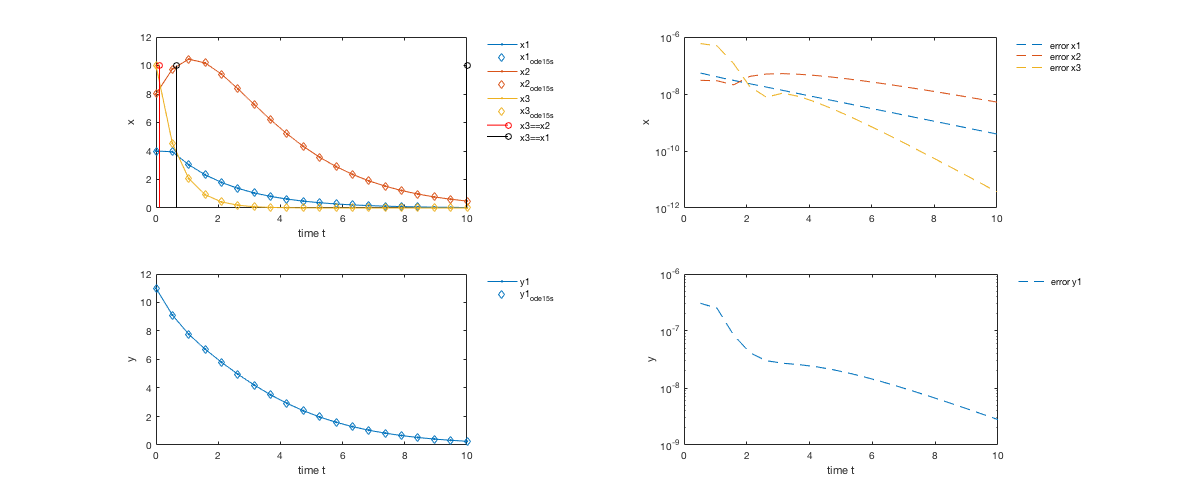
\includegraphics[width=\textwidth]{../../examples/example_events/html/example_events_01.png}
\begin{par}
FORWARD SENSITIVITY ANALYSIS
\end{par} \vspace{1em}
\begin{DoxyCode}
options.sensi = 1;

sol = simulate_model_events(t,log10(p),k,D,options);
\end{DoxyCode}
\begin{par}
FINITE DIFFERENCES
\end{par} \vspace{1em}
\begin{DoxyCode}
eps = 1e-4;
xi = log10(p);
for ip = 1:4;
    xip = xi;
    xip(ip) = xip(ip) + eps;
    solp = simulate_model_events(t,xip,k,D,options);
    sx_fd(:,:,ip) = (solp.x - sol.x)/eps;
    sy_fd(:,:,ip) = (solp.y - sol.y)/eps;
    sz_fd(:,:,ip) = (solp.z - sol.z)/eps;
end
\end{DoxyCode}
\begin{par}
PLOTTING
\end{par} \vspace{1em}
\begin{DoxyCode}
figure
for ip = 1:4
    subplot(4,2,ip*2-1)
    hold on
    for ix = 1:size(sol.x,2)
        plot(t,sol.sx(:,ix,ip),'.-','Color',c_x(ix,:))
        plot(t,sx_fd(:,ix,ip),'d','Color',c_x(ix,:))
    end
    legend('sx1','sx1_{fd}','sx2','sx2_{fd}','sx3','sx3_{fd}','Location','NorthEastOutside')
    legend boxoff
    title(['state sensitivity for p' num2str(ip)])
    xlabel('time t')
    ylabel('sx')
    box on

    subplot(4,2,ip*2)
    plot(t,abs(sol.sx(:,:,ip)-sx_fd(:,:,ip)),'--')
    legend('error sx1','error sx2','error sx3','Location','NorthEastOutside')
    legend boxoff
    title(['state sensitivity for p' num2str(ip)])
    xlabel('time t')
    ylabel('error')
    set(gca,'YScale','log')
    box on
end
set(gcf,'Position',[100 300 1200 500])

figure
for ip = 1:4
    subplot(4,2,ip*2-1)
    hold on
    for iy = 1:size(sol.y,2)
        plot(t,sol.sy(:,iy,ip),'.-','Color',c_x(iy,:))
        plot(t,sy_fd(:,iy,ip),'d','Color',c_x(iy,:))
    end
    legend('sy1','sy1_fd','Location','NorthEastOutside')
    legend boxoff
    title(['observable sensitivity for p' num2str(ip)])
    xlabel('time t')
    ylabel('sy')
    box on

    subplot(4,2,ip*2)
    plot(t,abs(sol.sy(:,:,ip)-sy_fd(:,:,ip)),'--')
    legend('error sy1','Location','NorthEastOutside')
    legend boxoff
    title(['error observable sensitivity for p' num2str(ip)])
    xlabel('time t')
    ylabel('error')
    set(gca,'YScale','log')
    box on
end
set(gcf,'Position',[100 300 1200 500])

figure
for ip = 1:4
subplot(4,2,2*ip-1)
bar(1:options.nmaxevent,sol.sz(1:options.nmaxevent,:,ip),0.8)
hold on
bar(1:options.nmaxevent,sz_fd(1:options.nmaxevent,:,ip),0.4)
legend('x3==x2','x3==x1','x3==x2 fd','x3==x1 fd','Location','NorthEastOutside')
legend boxoff
title(['event sensitivity for p' num2str(ip)])
xlabel('event #')
ylabel('sz')
box on

subplot(4,2,2*ip)
bar(1:options.nmaxevent,sol.sz(1:options.nmaxevent,:,ip)-sz_fd(1:options.nmaxevent,:,ip),0.8)
legend('error x3==x2','error x3==x1','Location','NorthEastOutside')
legend boxoff
title(['error event sensitivity for p' num2str(ip)])
xlabel('event #')
ylabel('sz')
box on
end
set(gcf,'Position',[100 300 1200 500])

drawnow
\end{DoxyCode}

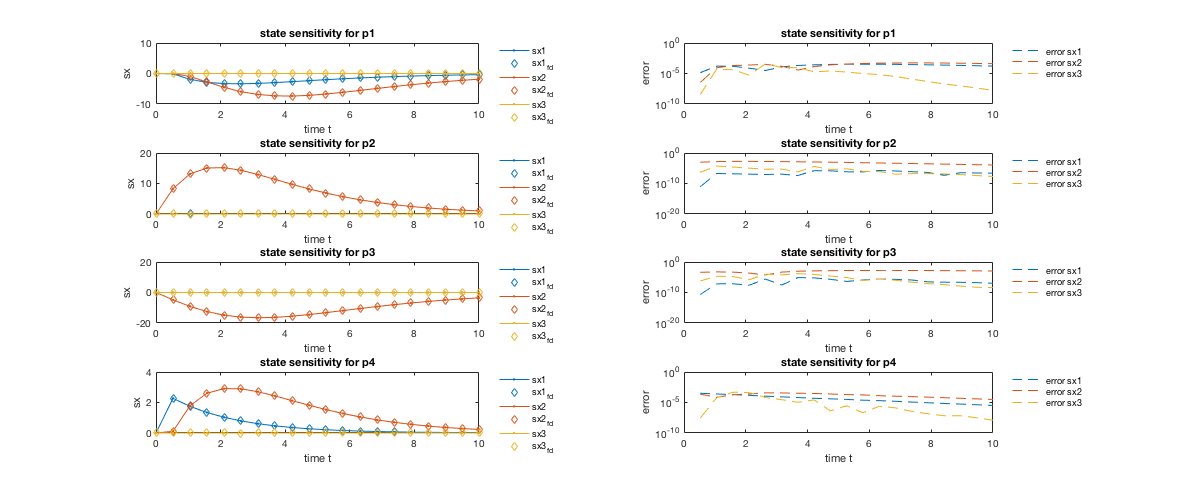
\includegraphics[width=\textwidth]{../../examples/example_events/html/example_events_02.png}

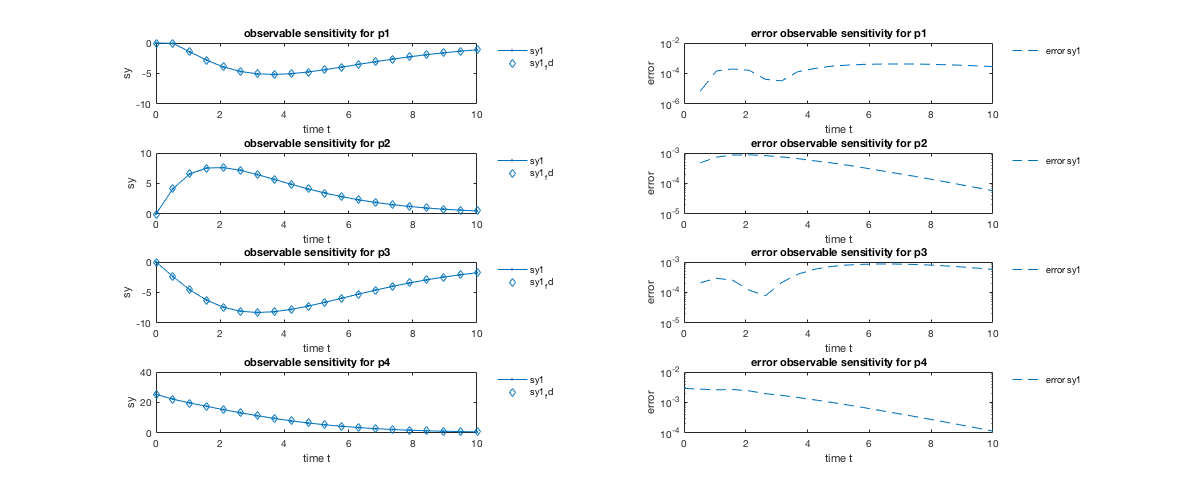
\includegraphics[width=\textwidth]{../../examples/example_events/html/example_events_03.png}

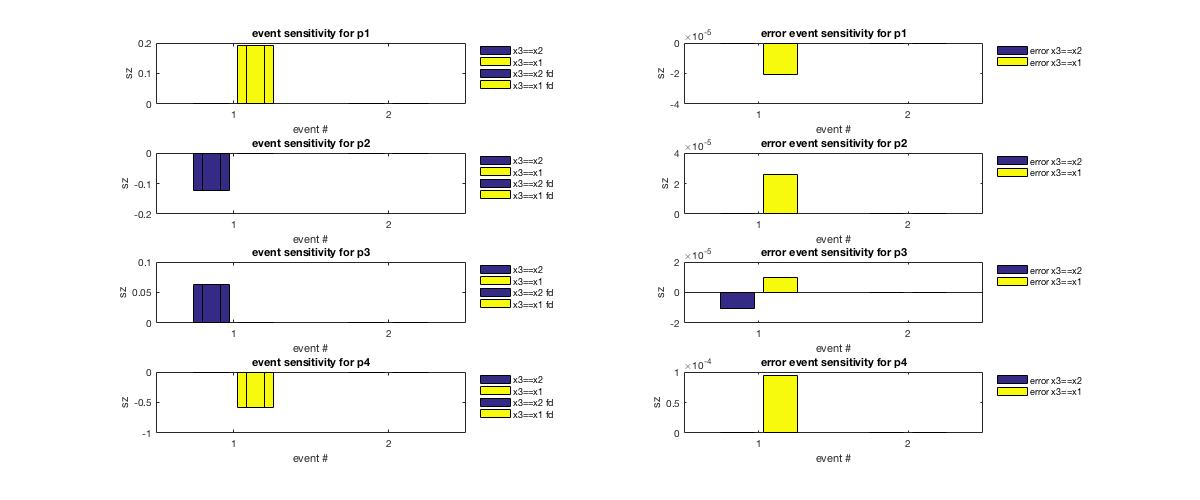
\includegraphics[width=\textwidth]{../../examples/example_events/html/example_events_04.png}
\begin{DoxyCode}
end
\end{DoxyCode}




    